\chapter{Anatomy}\label{ch:anatomy}

\chapterCoverImage{anatomy}

As with every practice dealing with the human body, a basic understanding of the human anatomy gives a tremendous advantage.
It will allow you to see and \textbf{experience} things differently, knowing about how your body is ``composed''.
The field is, of course, huge, thus it won't be necessary to go too much into details and focus on certain areas.
Yet an understanding of basic terminology is required to be able to \textbf{communicate} in this field.

\section{Terminology}\label{sec:terminology}

The wording used in anatomy/medicine is built from sub-elements (which usually originated from Latin), thus:
Learning first the elements, and then putting them together to be able to infer the meaning of more complex, compound terms.

\subsection{Orientation}

Because a person can stand, sit, lie, or be in all kinds of positions, it is necessary to have an absolute frame of reference to provide orientation instructions.
When someone uses simple language like ``up'' or ``front'', it is not entirely clear what is actually meant, thus the following anatomical terms lead to a more \textbf{non-ambiguous language}.

\begin{itemize*}
    \item \textbf{Anterior/posterior}: front/back
    \item \textbf{Ventral/dorsal}: front/back of the torso
    \item \textbf{Superior/inferior}: above/below
    \item \textbf{Cranial/caudal}: head-/tail-wards
    \item \textbf{Proximal/distal}: towards to/away from center
    \item \textbf{Medial/lateral}: towards/away from the midline
    \item \textbf{Superficial/profound}: more outside/inside the body
\end{itemize*}

\subsection{Movements}

Each body part can move in certain ways and directions based on the type of joint (see below) and how muscles pull on it.
Again, instructing someone to ``move up'' is ambiguous, whereas ``flex the right knee'' is clear as it can be.

\begin{itemize*}
    \item \textbf{Extension/flexion}: increase / decrease joint angle (stretch / bend)
    \item \textbf{Internal/external (medial/lateral) rotation}: rotating the arm / leg counter- / clockwise towards to / away from the body
    \item \textbf{Adduction/abduction}: moving towards / away from the midline
    \item \textbf{Elevation/depression}: moving the shoulder up / down
    \item \textbf{Pronation/supination}: forearm rotation palm facing up / down
    \item \textbf{Dorsi-/plantar-flexion}: move the ankle towards the dorsum (superior surface, up) or plantar (sole, down) also often called ``point''
    \item \textbf{In-/eversion}: sole towards / away from the median plane
    \item \textbf{Opposition/reposition}: thumb and little finger together / spread
    \item \textbf{Pro-/retraction}: anterolateral / posteromedial movement of the scapula (move shoulder forward/backward)
    \item \textbf{Circumduction}: conical (not really circular) movement of a limb extending from the joint it's moved by
\end{itemize*}

If we take for example a simple shoulder roll, it can be dissected in four movements: elevation, retraction, depression, and protraction.
Or similar with drawing circles with the toes, moving the ankle: dorsi-flexion, eversion, plantar-flexion, and inversion.

Terms derived from lateral movement include:

\begin{itemize*}
    \item \textbf{Uni-lateral}: ``\textit{unus}'' meaning ``one'', on one side of the body
    \item \textbf{Bi-lateral}: ``\textit{bis}'' meaning ``twice'', on both sides of the body
    \item \textbf{Homo-(Ipsi-)lateral}: ``\textit{ipse}'' meaning ``same''
    \item \textbf{Contra-lateral}: ``\text{contra}'' meaning ``against'', e.g. arm on one side, and leg on the other side, creating a diagonal, like we do while walking; also one hemisphere of the brain is controlling the other side of the body
\end{itemize*}

Sometimes the Latin word for left (``sinister'') and right (``dexter'') are being used instead.
Check the next time you have a medical report available, like an X-ray, and you will see these terms pop up; consider yourself a nerd from now on.

\section{Structures}\label{sec:structures}

Next to being familiar with the very basic words of positions and directions, we also need to be able to refer to concrete structures (bones and muscles).
Make yourself thus familiar with some (by far not all) anatomical terms, which help you further understand this medical jargon.

\subsection{Bones}\label{subsec:bones}

The human body has \textbf{206 bones} we can (usually) enumerate; yet by birth we have a few more, up to 280.
The head and trunk (the axial skeleton) make up 80 bones and the limbs (the appendicular skeleton) the other 126.
There are 27 bones for each hand (19 for phalanges plus metacarpals, and 8 carpals), and 26 for each foot (phalanges, metatarsals, and tarsals).

\begin{itemize*}
    \item \textbf{Atlas and axis}: two top most cervical vertebrae
    \item \textbf{Clavicle}: the collar bone connecting sternum and shoulder
    \item \textbf{Coccyx}: the tailbone; the last part of the spine
    \item \textbf{Cranium}: the skull (cervical = neck)
    \item \textbf{Patella}: the knee cap (olecranon is the elbow)
    \item \textbf{Processus}: a bulged out structure; usually tendons attach to it
    \item \textbf{Scapula}: the shoulder blade
    \item \textbf{Sacrum}: big triangular bone at the base of the spine
    \item \textbf{SIAS}: Prominent hip bone (Spina Illiaca Anterior Superior)
    \item \textbf{Vertebra}: An irregular bone forming the spine / vertebral column.
    \item \textbf{Sternum}: the chest bone
\end{itemize*}

For the sake of completeness, it is mentioned that we have true ribs (1-7, sternum connection), false ribs (8-10/12, cartilage), and floating ribs (11-12, no connection).
Also, the spine consists of 33 vertebra: 7 cervical, 12 thoracic, 5 lumbar, 5 fused sacral, and 4 fused forming the coccyx.

\subsection{Muscles}\label{subsec:muscles}

There are \textbf{between 600 and 840 muscles} within the typical human body, depending on how they are counted, and some variations due to mutations.

\begin{itemize*}
    \item \textbf{Abs}: abdominal muscles with 3 layers wrapped around the belly
    \item \textbf{Core muscles}: everything attached to the spine; not only the abs
    \item \textbf{Diaphragm}: muscle for breathing at the bottom of the ribs
    \item \textbf{Glutes}: buttocks consisting of maximus, medius, et minimus
    \item \textbf{Obliques}: part of the core, at the sides of the abs
    \item \textbf{Pectoralis}: the chest muscle (major and minor)
    \item \textbf{Pelvic floor}: similar to diaphragm but at the bottom of the torso
    \item ``\textbf{Stomach muscles}'': the stomach is an organ, which indeed has (involuntary) muscles, but it's located on the left side underneath the ribs, and should not be confused with the abs / lower belly!
    \item \textbf{Trapezius}: at top shoulder around the neck
    \item \textbf{Transverse}: part of the core, like a belt around it
\end{itemize*}

\section{Planes}\label{sec:planes}

\begin{wrapfigure}{R}{0.3\textwidth}
    \centering
    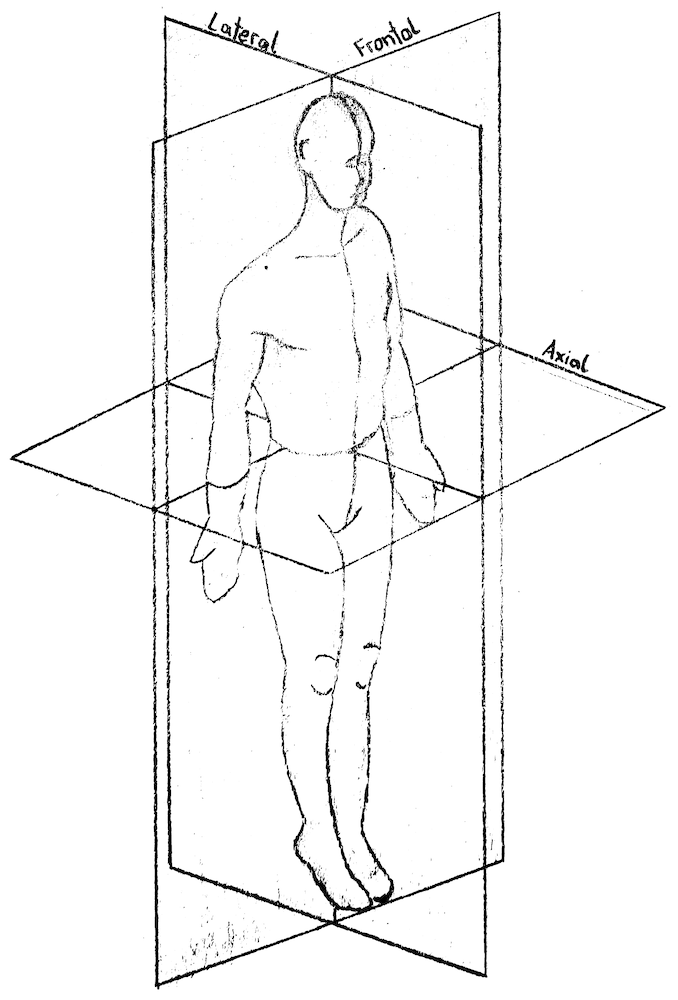
\includegraphics[width=0.3\textwidth]{images/anatomy/planes}
    \caption{The three anatomic \textbf{planes} for the human body.}
\end{wrapfigure}

We differentiate 3 different anatomical planes in which movement can happen:

\noindent \textbf{Frontal Plane}: Also called \textit{Coronal Plane} or \textit{Vertical Plane} and, not surprisingly, represents the plane when looking from the front of the body, dividing the body into an anterior/posterior part.
The directions can be medial/lateral, thus resulting in the movements of ad-/abduction, elevation/depression and in-/eversion.

\noindent \textbf{Lateral Plane}: Also called \textit{Sagittal Plane}, \textit{Longitudinal Plane} or \textit{Anteroposterior Plane}, which is going through the midline and shows the body when looking from the side, separating it into a left/right part.
The directions are thus anterior/posterior and movements are flexion/extension and pro-/retraction.

\noindent \textbf{Axial Plane}: Also called \textit{Transverse Plane}, \textit{Horizontal Plane} (the other two planes are vertical) or \textit{Cross-Sectional Plane}, and divides the body into a top/bottom part.
Directions are thus superior/inferior and allowing movements like rotation, supination/pronation and circumduction.

\section{Joints}\label{sec:joints}

Bones are connected through joints where muscles (together with tendons) can evoke movement.
For different movements, \textbf{different types} of (synovial) joints are needed:

\begin{itemize*}
    \item \textbf{Ball/Socket}: free movement; e.g. hip, shoulder
    \item \textbf{Pivot}: rotation; head (atlantoaxial), elbow (radioulnar)
    \item \textbf{Hinge}: flexion/extension; elbow (humeroulnar), knee
    \item \textbf{Saddle}: fingers-hand (trapeziometacarpal)
    \item \textbf{Condyloid}: fingers/wrist (metacarpophalangeal)
    \item \textbf{Plane}: hand (intercarpal) and feet (tarsal)
    \item \textbf{Gliding}: mini bones in feet
\end{itemize*}
